%%%%%%%%%%%%%%%%%%%%%%%%%%%%%%%%%%%%%%%%%
% Article Notes
% LaTeX Template
% Version 1.0 (1/10/15)
%
% This template has been downloaded from:
% http://www.LaTeXTemplates.com
%
% Authors:
% Vel (vel@latextemplates.com)
% Christopher Eliot (christopher.eliot@hofstra.edu)
% Anthony Dardis (anthony.dardis@hofstra.edu)
%
% License:
% CC BY-NC-SA 3.0 (http://creativecommons.org/licenses/by-nc-sa/3.0/)
%
%%%%%%%%%%%%%%%%%%%%%%%%%%%%%%%%%%%%%%%%%

%----------------------------------------------------------------------------------------
%	PACKAGES AND OTHER DOCUMENT CONFIGURATIONS
%----------------------------------------------------------------------------------------

\documentclass[
10pt, % Default font size is 10pt, can alternatively be 11pt or 12pt
a4paper, % Alternatively letterpaper for US letter
% twocolumn, % Alternatively onecolumn
% landscape % Alternatively portrait
]{report}

%%%%%%%%%%%%%%%%%%%%%%%%%%%%%%%%%%%%%%%%%
% Article Notes
% Structure Specification File
% Version 1.0 (1/10/15)
%
% This file has been downloaded from:
% http://www.LaTeXTemplates.com
%
% Authors:
% Vel (vel@latextemplates.com)
% Christopher Eliot (christopher.eliot@hofstra.edu)
% Anthony Dardis (anthony.dardis@hofstra.edu)
%
% License:
% CC BY-NC-SA 3.0 (http://creativecommons.org/licenses/by-nc-sa/3.0/)
%
%%%%%%%%%%%%%%%%%%%%%%%%%%%%%%%%%%%%%%%%%

%----------------------------------------------------------------------------------------
%	REQUIRED PACKAGES
%----------------------------------------------------------------------------------------

\usepackage[includeheadfoot,columnsep=2cm, left=1in, right=1in, top=.5in, bottom=.5in]{geometry} % Margins

\usepackage[T1]{fontenc} % For international characters
\usepackage{XCharter} % XCharter as the main font

\usepackage[english]{babel} % Use english by default

% maths packages

\usepackage{amsmath}
\usepackage{xfrac}
\usepackage{multirow}
\usepackage{float}
\usepackage{xcolor}
\usepackage{enumerate}
\usepackage{listings}
\usepackage{amsfonts}

%----------------------------------------------------------------------------------------
%	CUSTOM COMMANDS
%----------------------------------------------------------------------------------------

\newcommand{\articletitle}[1]{\renewcommand{\articletitle}{#1}} % Define a command for storing the article title

\newcommand{\datenotesstarted}[1]{\renewcommand{\datenotesstarted}{#1}} % Define a command to store the date when notes were first made
\newcommand{\docdate}[1]{\renewcommand{\docdate}{#1}} % Define a command to store the date line in the title

\newcommand{\docauthor}[1]{\renewcommand{\docauthor}{#1}} % Define a command for storing the article notes author

% Define a command for the structure of the document title
\newcommand{\printtitle}{
\begin{center}
\topskip0pt
\vspace*{\fill}
\textbf{\Huge{The Notes Project}}

\vspace{2ex}

\textbf{\huge{\articletitle}}

\vspace{1ex}

\Large\docdate \\
\vspace{1ex}
\Large\docauthor \\
\vspace*{\fill}

\end{center}
}

% \renewcommand{\theenumii}{\alph{enumii}.}

\usepackage{fancyhdr}

\newcommand{\ls}[2]{\sum_{#1=1}^{#2}}

\newcommand{\comment}[1]{%
  \text{\phantom{(#1)}} \tag{#1}
}

\newlength\dlf  % Define a new measure, dlf
\newcommand{\alignedbox}[2]{
% Argument #1 = before & if there were no box (lhs)
% Argument #2 = after & if there were no box (rhs)
&  % Alignment sign of the line
{\settowidth\dlf{#1}\addtolength\dlf{\fboxsep+\fboxrule} \hspace{-\dlf} \boxed{#1 #2}}
}
\newcommand{\Perm}[2]{{}^{#1}\!P_{#2}}%
\newcommand{\Comb}[2]{{}^{#1}C_{#2}}%

%----------------------------------------------------------------------------------------
%	STRUCTURE MODIFICATIONS
%----------------------------------------------------------------------------------------

\setlength{\parskip}{3pt} % Slightly increase spacing between paragraphs

% Uncomment to center section titles
\usepackage{sectsty}
\sectionfont{\centering}

% Uncomment for Roman numerals for section numbers
\renewcommand\thesection{\Roman{section}}


\usepackage{pifont}

\usepackage{tikz, pgfplots}
\pgfplotsset{compat=1.18}
\usetikzlibrary{positioning}

\usepackage{gensymb}


% ------------------------
%        PIE CHART
% ------------------------

\newcommand{\pieslice}[6][black!10]{
%%% Usage: \pieslice[color]{total}{start angle}{end angle}{data value}{label}
  % calculate start and end points of arc
  \pgfmathparse{#3/#2*360}
  \let\a\pgfmathresult
  \pgfmathparse{#4/#2*360}
  \let\b\pgfmathresult

  % calculate mid angle of arc
  \pgfmathparse{0.5*\a+0.5*\b}
  \let\midangle\pgfmathresult

  % draw slice
  \draw[fill=#1] (0,0) -- (\a:1) arc (\a:\b:1) -- cycle;

  % outer label
  \node[label=\midangle:{\small#6}] at (\midangle:1) {};

  % inner label
  \pgfmathparse{min((\b-\a-10)/110*(-0.3),0)}
  \let\temp\pgfmathresult
  \pgfmathparse{max(\temp,-0.5) + 0.8}
  \let\innerpos\pgfmathresult
  \pgfmathparse{(\b-\a)/3.6} % convert slice size to percentage
  \let\percentage\pgfmathresult
  \node at (\midangle:\innerpos) {\small\pgfmathprintnumber[fixed,precision=1]{\percentage}\%};
}

\newcommand{\pie}[2][{{"black!10"}}]{
%%% Usage: \pie[{colour palette array}]{{label/value array}}
  % init colour palette
  \pgfmathparse{dim(#1)} % find N of array
  \let\paletteDim\pgfmathresult
  \newcounter{colourIndex}

  % get total for dividing pie into sectors
  \newcounter{total}
  \foreach \val/\name in #2 {
    \addtocounter{total}{\val}
  }

  \newcounter{a}
  \newcounter{b}
  \foreach \val/\name in #2 {
    \setcounter{a}{\value{b}}
    \addtocounter{b}{\val}

    % get colour from palette
    \pgfmathparse{#1[\thecolourIndex]}
    \let\colour\pgfmathresult

    \pieslice[\colour]{\thetotal}{\thea}{\theb}{\val}{\name}

    % increment colour palette
    \stepcounter{colourIndex}
    \ifnum \thecolourIndex=\paletteDim \setcounter{colourIndex}{0}\fi
  }
}

\def\palette{{"blue!60","cyan!50","yellow!50","orange!60","red!60",
    "teal!50","brown!50!black!50","purple!50","lime!50!black!30"}}
    
    
% ---------------------------
%           TALLY
% ---------------------------

\newcount\tmpnum
\def\tallymarks#1{\leavevmode \lower1bp\vbox to9bp{}%
   \tmpnum=#1
   \loop \ifnum\tmpnum<5 \kern1bp \tallynum\tmpnum \else \tallyV \fi
         \advance\tmpnum by-5
         \ifnum\tmpnum>0 \repeat
}
\def\tallynum#1{\bgroup\tmpnum=#1\relax
   \loop \ifnum\tmpnum>0
         \kern1bp \tallyI \kern1bp
         \advance\tmpnum by-1
         \repeat
   \egroup
}
\def\tallyI{\pdfliteral{q .5 w 0 -1 m 0 8 l S Q}}
\def\tallyV{\kern1bp\pdfliteral{q .5 w -1 0 m 9 7 l S Q}\tallynum4\kern1bp }

 % Input the file specifying the document layout and structure

%----------------------------------------------------------------------------------------
%	ARTICLE INFORMATION
%----------------------------------------------------------------------------------------

\articletitle{Descriptive Statistics} % The title of the article

\datenotesstarted{December 9, 2023} % The date when these notes were first made
\docdate{\datenotesstarted; rev. \today} % The date when the notes were lasted updated (automatically the current date)

\docauthor{Keval Mehta, Divyansha Sachdeva} % Your name

%----------------------------------------------------------------------------------------

\begin{document}

\pagestyle{myheadings} % Use custom headers


%----------------------------------------------------------------------------------------
%	PRINT ARTICLE INFORMATION
%----------------------------------------------------------------------------------------

\thispagestyle{plain} % Plain formatting on the first page

\printtitle % Print the title

%----------------------------------------------------------------------------------------
%	ARTICLE NOTES
%----------------------------------------------------------------------------------------

\part{Descriptive Statistics - I} 

\section*{Syllabus}

\begin{itemize}
\item[] \textbf{Unit 1: Types of Data and Data Condensation}
\begin{enumerate}
\item Concept of population and sample. Different types of scales: nominal, ordinal, interval and ratio.
\item Collection of Primary data: concept of a questionnaire and a schedule, Secondary data
\item Types of data: Qualitative and quantitative data; Time series data and cross section data, discrete and continuous data.
\item Tabulation \& Diagrammatic representation using bar diagrams, Line diagram and pie chart.
\item Univariate frequency distribution of discrete and continuous variables. Cumulative frequency distribution.
\item Graphical representation of frequency distribution by Histogram, frequency polygon, Stem and leaf diagram and Cumulative frequency curve.
\end{enumerate}
\item[] \textbf{Unit 2: Measures of Central Tendency}
\begin{enumerate}
\item Concept of central tendency of data. Requirements of good measure
\item Mean, Median, Mode: Arithmetic mean (Simple, weighted mean,
combined mean), Geometric mean, Harmonic mean, Median, Mode,
Empirical relation between mean, median and mode
\item Partition Values: Quartiles, Deciles, Percentiles.
\item Merits and demerits of using different measures \& its applicability
\end{enumerate}
\item[] \textbf{Unit 3: Measures of Dispersion, Skewness \& Kurtosis}
\begin{enumerate}
\item Concept of dispersion. Requirements of good measure.
\item Absolute and Relative measures of dispersion: Range, Quartile
Deviation, Mean absolute deviation, Standard deviation.
\item Variance and Combined variance, raw moments and central moments
and relations between them.
\item Concept of Skewness and Kurtosis: Measures of Skewness: Karl
Pearson’s, Bowley’s and Coefficient of skewness based on moments.
\item Measure of Kurtosis
\item Box Plot
\end{enumerate}
\end{itemize}

% ---------------------------------------
%          Notes Start Here
% ---------------------------------------


\chapter*{Unit 1: Types of Data and Data Condensation}



\subsection*{What are statistics?}

There are two subdivisions of statistical method:
\begin{itemize}
\item Descriptive Statistics - It deals with the presentation of
numerical facts, or data, in either tables or graphs form,
and with the methodology of analysing the data.
\item Inferential Statistics - It involves techniques for making
inferences about the whole population on the basis of
observations obtained from samples.
\end{itemize}

\subsubsection*{Some Definitions}
\begin{description}
\item[Population] A population is the group from which data are to be collected. The entire group of individuals is called the population.
\item[Sample] Usually populations are so large that a researcher cannot examine the entire group. Therefore, a sample is selected to represent the population in a research study.
\item[Data] The measurements obtained in a research study are called the data. The goal of statistics is to help researchers organize and interpret the data.
\end{description}

\subsubsection*{Types of Statistical data}
\begin{itemize}
\item Primary data is data collected primarily for the purpose of
the given enquiry. They are original in character and are raw
materials of the enquiry.
\item Secondary data are data already collected by someone's for
some purpose and are available for the present study.
\end{itemize}

\subsection*{Primary Data Collection Methods}

\subsubsection*{Direct personal observation}
\begin{itemize}
\item In this method, the investigator collects the data personally.
\item They ask or cross-examine the informant in a tactful and courteous manner, and collect the necessary information.
\item This method is adopted when
\begin{itemize}
\item intensive or in-depth study is essential.
\item greater accuracy is needed.
\item the field of enquiry is not large but complex.
\item data of a confidential nature are to be collected.
\item sufficient time is available.
\end{itemize}
\item Such a personal enquiry gives reliable and accurate information as
response will be encouraging because of personal touch.
\item Also uniformity and homogeneity of data can be maintained.
\item However, such an enquiry will be expensive and time consuming \& will not give good results at the hands of an untrained investigator.
\item Also, the chances of personal prejudices/ bias creeping into the investigation are more.
\end{itemize}
\subsubsection*{Indirect oral investigation}
\begin{itemize}
\item This method is used when the informant is reluctant to supply
information.
\item Here the investigator approaches witnesses or third parties who are in touch with the informant. For instance if one wants to collect information about drinking or gambling habits of people
one gets the information from family members, friends and/or liquor shops, etc.
\item This method is generally adopted by Government agencies for
their enquiry committees of commissions.
\item Also, in cases of thefts, murders, riots etc. The police interrogate third parties who possess knowledge about the happenings under study.
\item This method is simple and convenient, and adequate information can be obtained if information is collected from different parties.
\item However, absence of direct contact can mar the reliability of the information.
\item Also, witnesses may colour the information to suit their interests.
\end{itemize}
\subsubsection*{Data through Mailed Questionnaires/Online Data Collection}
\textbf{A. Mailed Questionnaire}
\begin{itemize}
\item As the title suggests data is collected through a questionnaire consisting of a list of questions pertaining to the enquiry.
\item This questionnaire is posted to the respondents, who are expected to answer the questions or write the answers in the blank spaces. A covering letter is also sent along with the questionnaire requesting full co-operation and prompt reply from the respondents
\item This method is followed by research workers, private individuals, non-official agencies and Government agencies. The mailed questionnaire method is the most economical and there is a saving of time and labour. It is suitable when the area of the  survey is large.
\item Since information is obtained directly from respondents error in the investigation is small.
\item However, since there is no direct contact between investigator and respondent one can not be sure about the accuracy and reliability of the data.
\item Some people may not reply as they may be illiterate or simply lazy.
\item This could lead to non-response or delayed response.
\end{itemize}
\textbf{B. Online Data Collection}
\begin{itemize}
\item As the title suggests data is collected through a questionnaire consisting of a list of questions pertaining to the enquiry through an online method using internet.
\item This questionnaire/form is posted to the respondents, who are expected to answer the questions or write the answers in the blank spaces. A covering message is also sent along with the questionnaire requesting full co-operation and prompt reply from the respondents.
\item The methods used are Google Forms, Computer-Assisted Telephone Interviewing (CATI) etc.
\end{itemize}
\subsubsection*{Information through agencies}
\begin{itemize}
\item  Here, the investigator appoints agents or correspondents to collect data. These agents collect the information and transfer it to the investigator.
\item This method of primary data collection is usually followed by
news agencies where information is needed in different fields like
politics, sports, natural and man-made calamities etc.
\item This method is adopted where information is required from a
wide area on a regular basis.
\item Although this method gives extensive information in a speedy and economical way, it may be biased and the requisite degree of accuracy and uniformity can not be maintained.
\end{itemize}
\subsubsection*{Investigation through enumerators}
\begin{itemize}
\item This method is generally employed by the Government for popul
ation census etc.
\item A number of enumerators are selected and trained. They are then armed with standardised questionnaires and sent to informants to get first hand information.
\item This method is adopted when one requires reliable and accurate
information from all types of people (literate and illiterate).
\item However, this data collection exercise may be costly and time
consuming, and depends on the efficiency of the enumerators.
\end{itemize}

\subsection*{Questionnaires}
From the above primary data collection methods, the most important
requirement for a successful data collection exercise is a questionnaire. There are two sections in any questionnaire. They are:
\begin{description}
\item[Classification] This section includes the details of the respondents such as name, age, sex, education, marital status, occupation. Additionally, details like the date of interview and name of the interviewer are included in this section.
\item[Subject Matter] This section includes questions related to the subject matter of the inquiry. The answers given here can be analysed according to the information in the classification section
\end{description}

\subsubsection*{Requisites of a Good Questionnaire}
\begin{itemize}
\item The questionnaire must be brief, i.e. the number of questions
should be as few as possible as respondents will not like or may not have time for answering a long questionnaire. All the questions must be relevant to the problem under investigation
\item Questions should not be ambiguous. They must be capable of
one and only one interpretation.
\item Questions must be easily understood. Technical terms
must be avoided except when addressed to specialists.
\item Questions must be arranged in a logical sequence
\item Questions should have a precise answers. The answers should take the form of ‘yes’ or ‘no’, a quantity, a date, a place etc. Wherever possible the questionnaire should suggest answers so that the informant has merely to tick or cross (\ding{51} or \ding{55}) the answer.
\item Questions must not contain words of vague meaning. To ask if something is large or if a man is unskilled are examples of such questions.
\item Questions of a sensitive or personal nature should be avoided. Such questions may not be answered and some informants may be offended.
\item Questions should not require the respondent to make any
calculations. The figures provided by the respondent must
be accepted and calculations according to the need of the
questionnaire done later.
\item To check reliability of answers. Some questions should be
asked so as to provide cross-check for the answers to the
similar questions.
\end{itemize}

\subsubsection*{Schedules}
\begin{itemize}
\item This method of data collection is very much like the collection of data through questionnaire, with little difference which lies in the fact that schedules (proforma containing the set of questions) are filled in by the enumerators who are specially appointed for the purpose.
\item These enumerators go to respondents, put to them the questions from the schedule and record the replies in the space meant for the same in the proforma.
\item The method require careful selection of enumerators for filling up schedules and they should be trained to perform their job well. The enumerators should be honest, sincere, hardworking and should have patience and perseverance.
\item This method of data collection is very useful in extensive enquiries and can lead to fairly reliable results.
\item It is, however very expensive.
\item Population census all over the world is conducted through this method.
\end{itemize}

\subsubsection*{Differences Between Questionnaires and Schedules}
\begin{center}
\centering
\begin{tabular}{| p{0.49\textwidth} | p{0.49\textwidth} |}
\hline
Questionnaire & Schedule \\
\hline \hline 
Sent through mail to informants with a covering letter. & Filled in by the enumerator \\
\hline
Relatively \textbf{cheap} and economical, since we have to spend money only in preparing the questionnaire and mailing it to the respondents. No field staff is required. & Relatively \textbf{more expensive} since a considerable amount of money is spent in appointing enumerators and training them. \\
\hline
Non-response is high in case of questionnaire as many people do not respond, and many return questionnaire without answering all questions. & Non-response is generally very low in case of schedules. \\
\hline
The questionnaire method is likely to be \textbf{slow} since many respondents may not return the questionnaire on time. &
In case of schedule the information is \textbf{collected well in time} as they are filled in by the enumerators. \\
\hline
Questionnaire method can be used only when the respondents are literates and co-operative. & in case of schedules, the information can be gathered even when the respondents happen to be illiterate. \\
\hline
It is not clear as to who replies. & The identity of respondent is known. \\
\hline
\end{tabular}
\end{center}

\subsection*{Editing the Data}
\begin{itemize}
\item Once the data has been obtained either from primary or a
secondary source, the next step in any statistical investigation
is to edit data.
\item The main purpose of editing the data is to scrutinize it for
possible errors and irregularities.
\item The task of editing is a highly specialised one and necessary
too before proceeding to tabulation.
\item It requires great care, and negligence in this regard render a valuable study useless.
\end{itemize}

\subsubsection*{The Process}
\begin{itemize}
\item Check if the schedules/questionnaire for completeness:
The editor must see whether answer to each question has been furnished. If not, the informant must be contacted again. If one doesn't still get any reply then editor should mark 'no reply' in space provided for the answer.
\item Ensuring that there are no inconsistent entries:
The editor must check if answers to questions are not contradictory.
\item For example, if answers to two questions 'are you married?' and 'how many children do you have?' are 'no' and 'two' respectively, then clarification should be used.
\item Checking the questionnaires for accuracy:
Validity or reliability of conclusions drawn from survey depends on
accuracy of information. e.g. shifting of a decimal point. Also it is obvious that son’s age can not be 20 if the mother’s age is reported as 25. Entries reported for Sep 31 or Feb 30 cannot be considered.
\item Checking the questionnaire for homogeneity of answers: The editor must check if the questions have been interpreted uniformly. \item e.g. Gross pay vs. net pay or monthly pay vs. annual pay.
\end{itemize}


\subsubsection*{Types of Data}
The data can be of the following types:
\begin{itemize}
\item[\textbf{1}]
\begin{itemize}
\item Geographical or Spatial
\item Chronological or Time-Series
\end{itemize}
\item[\textbf{2}]
\begin{itemize}
\item Qualitative
\item Quantitative
\end{itemize}
\item[\textbf{3}]
\begin{itemize}
\item Discrete
\item Continuous
\end{itemize}
\end{itemize}


\subsection*{Measuring Variables}
\begin{itemize}
\item To establish relationships between variables, researchers must observe the variables and record their observations. This requires that the variables be \textbf{measured}.
\item The process of measuring a variable requires a set of categories called a \textbf{scale of measurement} and a process that classifies each individual into one category.
\end{itemize}

\begin{description}
\item[Nominal]
\begin{itemize}
\item[]
\item A nominal scale is an unordered set of categories identified only by name.
\item Measurement is done only in terms of whether the individual terms belong to some distinctively different categories
\item We cannot quantify or even rank order these categories.
\item Each category can be assigned a number (group 1, group 2 etc.). The assignment of numbers to qualitative classes is purely arbitrary since any number would do as well as another
\item The characteristic measured on nominal scale generates categorical data.
\item[\textbf{e.g.}] Data on gender, race, colour, city, etc.
\end{itemize}
\item[Ordinal]
\begin{itemize}
\item[]
\item An ordinal scale is an ordered set of categories.
\item This scale allows us to rank the items according to the classes but the differences between the adjacent ranks may not be equal.
\item It can be said that one class is higher than the other.
\item Ordinal measurements tell you the direction of difference between two individuals.
\item Nominal measurement provides less information than ordinal measurements.
\item[\textbf{e.g.}]  Socioeconomic status of families: Upper Class, Middle Class and Lower Class
\end{itemize}
\item[Interval]
\begin{itemize}
\item[]
\item An interval scale is an ordered series of equal-sized categories.
\item Interval variables allow us not only to rank order the items that are measured but also to quantify and capture the sizes of differences between them.
\item There is no true(absolute) zero.
\item The Fahrenheit scale is an example of interval scale.
\item An increase in temperature from 30\degree \ to 40\degree \  involves the same increase in temperature from 60\degree \ to 70\degree. Equal temperature differences are equal in the sense that the same amount of heat is required to raise the temperature of an object from 30\degree \ to 40\degree \ , or 60\degree \ to 70\degree \ . But \sfrac{\text{60}\degree}{\text{30}\degree} \(= \text{2}\) need not imply that 60\degree \  is twice as hot as 30\degree \  i.e. the ratio has no significance.
\item Unlike nominal and ordinal, it is a truly quantitative scale.
\item There is a constant (equal) size interval between any adjacent units on the measurement scale (unit distance) e.g. the difference between 40\degree \ 
and 30\degree \  is same as that between 70\degree \ \& 60\degree \ .
\item the existence of zero but does not necessarily indicate absence of quantity being measured (0\degree \  Fahrenheit does not necessarily mean absence of heat).
\item Some interval scales in biological data collection are circular scales (time of the day or time of a year where zero is arbitrary).
\item There is no inherent starting point and ratios are meaningless.
\item[\textbf{e.g.}] temperatures, time or pressure
\end{itemize}
\item[Ratio]
\begin{itemize}
\item[]
\item A ratio scale features an identifiable absolute zero point
\item It is an interval scale where a value of zero indicates none of the variable.
\item Ratio measurements identify the direction and magnitude of differences and allow ratio comparisons of measurements.
\item Most statistical data analysis procedures do not distinguish between the interval and ratio properties of the measurement scales.
\item In a ratio scale, both differences and ratios are meaningful.
\item There is a constant (equal) size interval between any adjacent units on the measurement scale (unit distance)
\item There is a True Zero Point. This enables us to say something about the ratio of measurements. E.g. A person weighing 100 kgs weighs double another weighing 50 kgs.
\item[\textbf{e.g.}] weight, height or distance
\end{itemize}
\end{description}

\subsubsection*{Analyses for Different Scales}
\begin{itemize}
\item Statistical analysis of the data depends on the scale of measurement.
\item For nominal scale, mode is the appropriate measure of central tendency and the \(\chi^2\) test is used for statistical significance.
\item In case of ordinal scale, the appropriate measures of central tendency and dispersion are median and quartile deviation. The tests of statistical significance are restricted to non-parametric tests.
\item For interval and ratio scales, the appropriate measures of central tendency and dispersion are mean and standard deviation respectively. The tests for statistical significance are \(t\)-test, \(F\)-test etc.
\end{itemize}

\subsection*{Classification of Data}

\subsubsection*{Why?}
\begin{itemize}
\item To condense raw data into a compact form which is easily understood and can be quickly interpreted.
\item To bring uniformity in large mass of data.
\item To facilitate comparison of two or more characteristics presented.
\end{itemize}

\begin{figure}[h!]
\centering
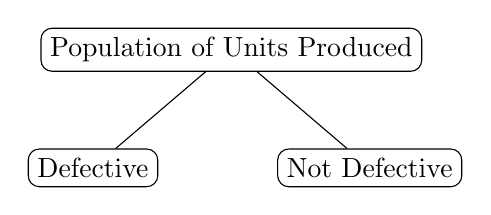
\begin{tikzpicture}
    [
      sibling distance=10em, 
      every node/.style = {shape=rectangle, rounded corners, draw, align=center, ->}
    ]

    \node{Population of Units Produced}
      child {node{Defective}}
      child {node{Not Defective}
            };
\end{tikzpicture}
\caption{One-Way Classification}
\label{fig:oneway}
\end{figure}

\begin{figure}[h!]
\centering
  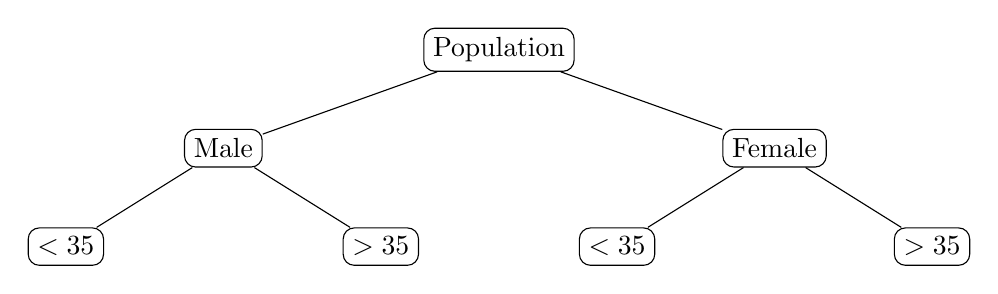
\begin{tikzpicture}
    [
      % sibling distance=20em, 
      every node/.style = {shape=rectangle, rounded corners, draw, align=center, ->},
      level 1/.style = {sibling distance=7cm},
      level 2/.style = {sibling distance=4cm}, 
      level 3/.style = {sibling distance=2cm}, 
      level distance = 1.25cm
    ]

    \node{Population}
      child {node{Male} 
              child{node{\(< 35\)}} 
              child{node{\(> 35\)}}
                    }
      child {node{Female} 
              child{node{\(< 35\)}} 
              child{node{\(> 35\)}}
            };
  \end{tikzpicture}
\caption{Manifold Classification}
\label{fig:manifold}
\end{figure}
            
\subsection*{Tabulation}

Tabulation may be defined as a logical and
systematic arrangement of statistical data in
rows and columns.

\subsubsection*{Why?}
\begin{itemize}
\item To simplify complex data
\item To clarify the aim of the survey
\item To do away with unnecessary details and save space
\item To make comparisons easy
\item To facilitate statistical analysis
\item To facilitate future studies in same or relevant field
\item To identify trends or patterns of data
\end{itemize}

A statistical table is a systematic presentation of numerical data in rows and columns with respect to some characteristics of the population.

\subsubsection*{Requirements of a good statistical table}
\begin{description}
\item[Title] Each table must have a title
displayed in bold type at the top of the table. It must
be brief and self-explanatory.
\item[Number] For easy reference of information in
the table, it must be numbered. The number can be
put at the top above the title or at the bottom.
\item [Stubs and Captions] Stubs are row headings and
captions are the column headings. These headings
should be well-defined and brief.
\item[Body] It is the most important part of any
table. It contains numerical information including
meaningful row and column totals.
\item[Source-Note] It mentions the source/origin of
information used in table.
\item[Footnote] Normally placed at the bottom of table, it gives explanation or elaboration about any information used in table.
\end{description}

\subsubsection*{Simple and Complex Tables}
\begin{itemize}
\item Simple and Complex tables are tables used to represent one or more characteristics under study.
\item In simple table the data are classified according to only one characteristic.
\item In a complex table two or more characteristics are shown.
\end{itemize}

\subsubsection*{Classifying statistical tables}
\begin{description}
\item[General Purpose]
\begin{itemize}
\item[]
\item General purpose tables are tables published by the Government and International bodies.
\item They are used as reference tables and they provide information about facts.
\item They are constructed to keep a record of the data collected as in census.
\end{itemize}
\item[Special Purpose]
\begin{itemize}
\item[]
\item Special purpose tables, also called summary tables are constructed to suit a particular purpose.
\item They are analytical in nature or derived from general purpose tables.
\end{itemize}
\end{description}

\begin{table} % oneway
\begin{center}
\begin{tabular}{| c | c |}
\hline
Department & No. of Employees \\
\hline \hline
R\&D & 9 \\
\hline
HR & 13 \\
\hline
Marketing & 19 \\
\hline
Finance & 12 \\
\hline
Sales & 7 \\
\hline
\hline
\textbf{Total} & 60 \\
\hline
\end{tabular}
\end{center}
\caption{A Simple Table}
\label{tab:simple}
\end{table}

\begin{table}[] %twoway
\begin{center}
\begin{tabular}{|cl|ccc|}
\hline
\multicolumn{2}{|c|}{\multirow{2}{*}{Department}} & \multicolumn{3}{c|}{No. of Employees}                           \\ \cline{3-5} 
\multicolumn{2}{|c|}{}                            & \multicolumn{1}{c|}{Male} & \multicolumn{1}{c|}{Female} & Total \\ \hline \hline
\multicolumn{2}{|c|}{R\&D}                        & \multicolumn{1}{c|}{6}    & \multicolumn{1}{c|}{3}      & 9     \\ \hline
\multicolumn{2}{|c|}{HR}                          & \multicolumn{1}{c|}{8}    & \multicolumn{1}{c|}{5}      & 13    \\ \hline
\multicolumn{2}{|c|}{Marketing}                   & \multicolumn{1}{c|}{10}   & \multicolumn{1}{c|}{9}      & 19    \\ \hline
\multicolumn{2}{|c|}{Finance}                     & \multicolumn{1}{c|}{8}    & \multicolumn{1}{c|}{4}      & 12    \\ \hline
\multicolumn{2}{|c|}{Sales}                       & \multicolumn{1}{c|}{4}    & \multicolumn{1}{c|}{3}      & 7     \\ \hline \hline
\multicolumn{2}{|c|}{\textbf{Total}}              & \multicolumn{1}{c|}{36}   & \multicolumn{1}{c|}{24}     & 60    \\ \hline
\end{tabular}
\end{center}
\caption{A Complex Table (Two-Way)}
\label{tab:complex_twoway}
\end{table}

\begin{table}[] %threeway
\begin{center}
\begin{tabular}{|cl|cccccccc|c|}
\hline
\multicolumn{2}{|c|}{\multirow{3}{*}{Department}} &
  \multicolumn{8}{c|}{No. of Employees} &
  \multirow{3}{*}{Grand Total} \\ \cline{3-10}
\multicolumn{2}{|c|}{} &
  \multicolumn{3}{c|}{Male} &
  \multicolumn{3}{c|}{Female} &
  \multicolumn{2}{c|}{Total} &
   \\ \cline{3-10}
\multicolumn{2}{|c|}{} &
  \multicolumn{1}{c|}{\(<\) 35} &
  \multicolumn{1}{c|}{\(>\) 35} &
  \multicolumn{1}{c|}{Total} &
  \multicolumn{1}{c|}{\(<\) 35} &
  \multicolumn{1}{c|}{\(>\) 35} &
  \multicolumn{1}{c|}{Total} &
  \multicolumn{1}{c|}{\(<\) 35} &
  \(>\) 35 &
   \\ \hline
\multicolumn{2}{|c|}{R\&D} &
  \multicolumn{1}{c|}{3} &
  \multicolumn{1}{c|}{3} &
  \multicolumn{1}{c|}{6} &
  \multicolumn{1}{c|}{2} &
  \multicolumn{1}{c|}{1} &
  \multicolumn{1}{c|}{3} &
  \multicolumn{1}{c|}{5} &
  4 &
  9 \\ \hline
\multicolumn{2}{|c|}{HR} &
  \multicolumn{1}{c|}{6} &
  \multicolumn{1}{c|}{2} &
  \multicolumn{1}{c|}{8} &
  \multicolumn{1}{c|}{2} &
  \multicolumn{1}{c|}{3} &
  \multicolumn{1}{c|}{5} &
  \multicolumn{1}{c|}{8} &
  5 &
  13 \\ \hline
\multicolumn{2}{|c|}{Marketing} &
  \multicolumn{1}{c|}{7} &
  \multicolumn{1}{c|}{3} &
  \multicolumn{1}{c|}{10} &
  \multicolumn{1}{c|}{6} &
  \multicolumn{1}{c|}{3} &
  \multicolumn{1}{c|}{9} &
  \multicolumn{1}{c|}{13} &
  6 &
  19 \\ \hline
\multicolumn{2}{|c|}{Finance} &
  \multicolumn{1}{c|}{5} &
  \multicolumn{1}{c|}{3} &
  \multicolumn{1}{c|}{8} &
  \multicolumn{1}{c|}{3} &
  \multicolumn{1}{c|}{1} &
  \multicolumn{1}{c|}{4} &
  \multicolumn{1}{c|}{8} &
  4 &
  12 \\ \hline
\multicolumn{2}{|c|}{Sales} &
  \multicolumn{1}{c|}{4} &
  \multicolumn{1}{c|}{0} &
  \multicolumn{1}{c|}{4} &
  \multicolumn{1}{c|}{2} &
  \multicolumn{1}{c|}{1} &
  \multicolumn{1}{c|}{3} &
  \multicolumn{1}{c|}{6} &
  1 &
  7 \\ \hline
\multicolumn{2}{|c|}{\textbf{Total}} &
  \multicolumn{1}{c|}{25} &
  \multicolumn{1}{c|}{11} &
  \multicolumn{1}{c|}{36} &
  \multicolumn{1}{c|}{15} &
  \multicolumn{1}{c|}{9} &
  \multicolumn{1}{c|}{24} &
  \multicolumn{1}{c|}{40} &
  20 &
  60 \\ \hline
\end{tabular}
\end{center}
\caption{A Complex Table (Three-Way)}
\label{tab:complex_threeway}
\end{table}

\subsection*{Diagrammatical Presentation of Data}

\subsubsection*{Why?}
\begin{itemize}
\item Besides tabulation, data can also be understood better if it was presented with the help of a diagram or a graph.
\item Cold figures may not be very inspiring to people but diagrams help us see the pattern and shape of the data.
\item Diagrams are a visual device to present data and they appeal to a layman too.
\end{itemize}

We use the following:
\begin{description}
\item[One Dimensional]
\begin{itemize}
\item[]
\item Bar Diagram
\begin{itemize}
\item Simple
\begin{itemize}
\item A simple bar diagram is a bar diagram used to represent one variable
\item For example – figures of sales, population (for various years, countries)
\item Simple bar diagram is the most common type of diagram used in practice
\item This diagram consists of vertical/horizontal bars of uniform width and height proportional to the value of the variable which the diagram seeks to present
\item It is called one-dimensional as it is only the height of the bar that matters and not the width
\item The space between the neighbouring bars must be uniform
\item Bars can be vertical or horizontal, but vertical bars are preferred as they are easier to comprehend and convenient for comparison
\end{itemize}
\item Subdivided
\begin{itemize}
\item This diagram is used where a variable is divided into different components and changes in the values of these components as well change in the value of a variable are important
\item Each bar gives a comparative study
\item The bar is subdivided into different components
\item Each component occupies a part of the bar proportional to its share in the total
\item To distinguish different components from one another different colours or patterns are used
\item Here a key to the diagram is absolutely essential
\item The subdivisions of the bar are either in absolute figures or as percentages of the whole
\item If percentages are used, then the diagram is called a percentage sub-divided bar diagram
\item Here, all the bars are of the same height
\end{itemize}
\item Multiple
\begin{itemize}
\item Multiple bar diagram is used to represent two or more sets of values which are related
\item The bars of the different sets are drawn adjacent to each other and the heights of the bars are proportional to the values
\item To distinguish between adjacent bars, different colours or patterns are used
\item Here, a key to the diagram is essential
\item This diagram can be used to represent different variable or one variable when the variable is divided into different components and the changes in the value of these components separately are important rather than the change in value of variable as a whole
\end{itemize}
\end{itemize}
\item Line Diagram
\begin{itemize}
\item A style of chart that is created by connecting a series of data points together with a line
\item This is the most basic type of chart used in finance and it is generally created by  connecting a series of past prices together with a line
\end{itemize}
\end{itemize}
\item[Two Dimensional]
\begin{itemize}
\item[]
\item Pie Diagram
\begin{itemize}
\item A pie diagram is a circle which represents the total value of a variable
\item The circle is divided into a number of sectors representing different components of the variable
\item These sectors are such that their areas are proportional to the values of the components i.e. the angles of the sectors are taken proportional to the values of the components
\item \(\text{Angle of each sector} = \frac{\text{Value of the component}}{\text{Total}} \times 360\)
\item The radius of the circle is taken proportional to the square-root of the total
\item The diagram is so called because it looks like a pie and the components resemble slices cut from it
\end{itemize}
\item Square Diagram
\item Rectangular Diagram
\end{itemize}
\item[Other]
\begin{itemize}
\item[]
\item Stem and Leaf Diagram
\end{itemize}
\end{description}

\begin{center}
\textbf{A Few Bar, Line, and Pie Graphs}
\end{center}
  \begin{minipage}{\linewidth}
      \centering
      \begin{minipage}{0.3\linewidth}
          \begin{figure}[H]
\pgfplotstableread{
0 35569
1 30428
2 32920  
3 16462 
}\dataset
\begin{tikzpicture}
\begin{axis}[ybar,
		axis lines=left,
        width=\textwidth,
        xmin=-0.5,
        xmax=3.5,
        ymin=0,
        ymax=50000,   
        xlabel=\(x\),     
        ylabel=\(y\),
        xtick=data,
        xticklabels = {
        		1, 2, 3, 4
        },
        major x tick style = {opacity=0},
        minor x tick num = 1,
        minor tick length=2ex,
        ]
\addplot[draw=black,fill=black!20] table[x index=0,y index=1] \dataset; %Data1
\end{axis}
 \end{tikzpicture}
 \caption{Simple Bar}
 \label{fig:simplebar}
\end{figure}
      \end{minipage}
      \hspace{0.03\linewidth}
      \begin{minipage}{0.3\linewidth}
          \begin{figure}[H]

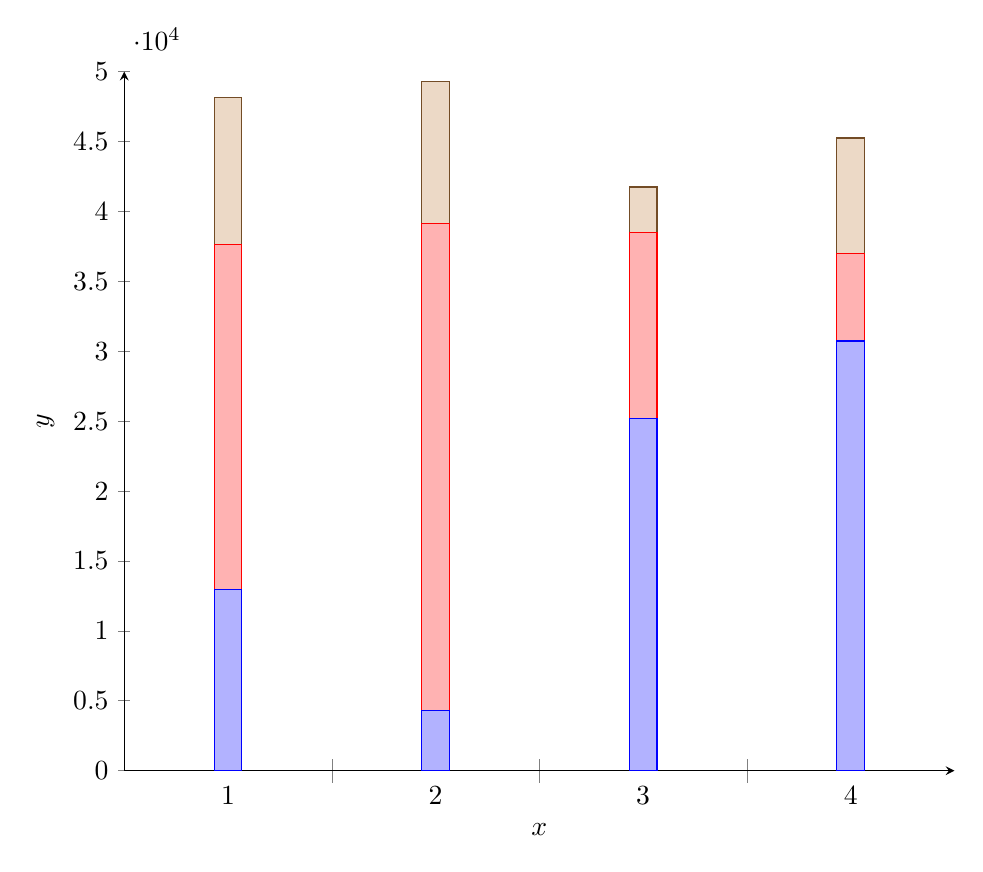
\begin{tikzpicture}
\begin{axis}[ybar stacked,
        axis lines=left,
        width=\textwidth,
        xmin=0.5,
        xmax=4.5,
        ymin=0,
        ymax=50000,   
        xlabel=\(x\),     
        ylabel=\(y\),
        xtick=data,
        xticklabels = {
        		1, 2, 3, 4
        },
        major x tick style = {opacity=0},
        minor x tick num = 1,
        minor tick length=2ex,
        ]
 
\addplot coordinates
{(1, 12983) (2, 4301) (3, 25192) (4, 30736)};
\addplot coordinates
{(1, 24639) (2, 34810) (3, 13281) (4, 6283)};
\addplot coordinates
{(1, 10538) (2, 10174) (3, 3283) (4, 8239)};

\end{axis}
 \end{tikzpicture}
 \caption{Subdivided Bar}
 \label{fig:subdividedbar}
\end{figure}
      \end{minipage}
      \hspace{0.03\linewidth}
     \begin{minipage}{0.3\linewidth}
          \begin{figure}[H]
\pgfplotstableread{
0 35569 8842
1 30428 4689
2 32920 6207  
3 16462 7562
}\dataset
\begin{tikzpicture}
\begin{axis}[ybar,
        axis lines=left,
        width=\textwidth,
        xmin=-0.5,
        xmax=3.5,
        xmin=-0.5,
        xmax=3.5,
        ymin=0,
        ymax=50000,   
        xlabel=\(x\),     
        ylabel=\(y\),
        xtick=data,
        xticklabels = {
        		1, 2, 3, 4
        },
        major x tick style = {opacity=0},
        minor x tick num = 1,
        minor tick length=2ex,
        ]
\addplot[draw=black,fill=black!20] table[x index=0,y index=1] \dataset; %Data1
\addplot[draw=black,fill=black!40] table[x index=0,y index=2] \dataset; %Data2
\end{axis}
 \end{tikzpicture}
 \caption{Multiple Bar}
 \label{fig:multiplebar}
\end{figure}
      \end{minipage}
  \end{minipage}
  
 

\begin{minipage}{\linewidth}
\centering
\begin{minipage}{0.45\linewidth}
\begin{figure}[H]
\begin{tikzpicture}
    \begin{axis}[
        xlabel=$x$,
        ylabel=$y$,
        xmin=0, xmax=30,
        ymin=0, ymax=100,
        xtick={10,20,30},
        ytick={10,20,30,40,50,60,70,80,90,100}
        ]
    \addplot[mark=*,blue] plot coordinates {
        (3,10)
        (8,30)
        (16,40)
        (20, 60)
        (27, 83)
    };
   \end{axis}
\end{tikzpicture}
\caption{Line}
\label{fig:line}
\end{figure}
\end{minipage}
\hspace{0.05\linewidth}
\begin{minipage}{0.45\linewidth}
\begin{figure}[H]
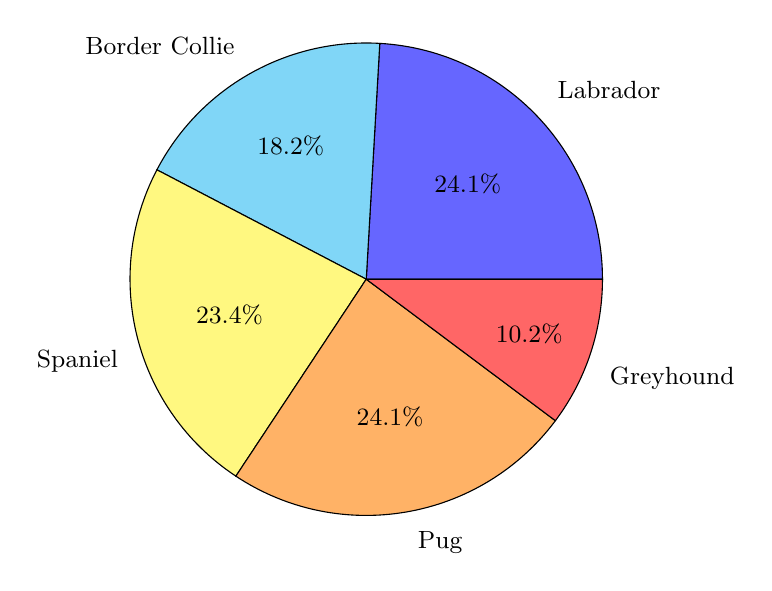
\begin{tikzpicture}[scale=3]
\pie[\palette]{{66/Labrador, 50/Border Collie, 64/Spaniel, 66/Pug, 28/Greyhound}}
\end{tikzpicture}
\caption{Pie}
\label{fig:pie}
\end{figure}
\end{minipage}
\end{minipage}

\subsubsection*{Advantages and Limitations}
\begin{description}
\item[Advantages]
\begin{itemize}
\item[]
\item It is easily understood by all including people who have no background of statistics
\item Data can be presented in a more attractive form and is appealing to the eye
\item Comparative analysis and interpretation is possible
\end{itemize}
\item[Limitations]
\begin{itemize}
\item[]
\item Diagrams do not show all the facts in detail
\item It is a supplement to tabular representation but not an alternative to it
\item The uses of certain diagrams are limited to
experts
\item If there is a wide gap between two different measurement, diagrams will not give a
meaningful look
\end{itemize}
\end{description}

\subsection*{Frequency Distributions}
\begin{itemize}
\item The collected data (after editing) is
called raw data
\item The raw data is in an ungrouped form i.e. the observations on the variate are just a set of numbers
\item We need to put them in the form of a table for better understanding
\item Such a table consists of two columns:
\begin{itemize}
\item classes
\item class frequency,
\end{itemize}
which denotes number of observations belonging to
each class.
\item Classes can be of three kinds:
\begin{itemize}
\item a discrete set of values
\item[e.g.] \(0, 1, 2, \dots\)
\item a discontinuous (inclusive) set of class intervals
\item[e.g.] \(0-9, 10-19, \dots\)
\item a continuous (exclusive) set of class intervals
\item[e.g.] \(0-10, 10-20, \dots\)
\end{itemize}
\item Sometimes, for statistical analysis, exclusive type of class intervals are required.
\item Hence, if the given frequency table is of inclusive type, it can be converted into exclusive type as follows:
\begin{enumerate}
\item Find the difference between the lower limit of a class and the upper limit of an earlier class
\item Subtract half of the difference from every lower class limit and add it to every upper class limit
\end{enumerate}
\end{itemize}

\subsubsection*{Example Calculation}

\textbf{Question:} The following data is about rainfall (in mms) in the month of July in a certain place. Prepare a frequency table taking class intervals \((40-50), (50-60),\dots\)

57.6, 72.8, 48.1, 71.4, 83.1, 91.6, 71.3, 63.4, 43.9, 69.2, 87.5, 90.1, 98.8, 49.2, 54.6, 71.5, 62.7, 59.7, 48.3, 54.1, 73.6, 48.2, 54.6, 77.1, 49.6, 58.3, 60.5, 63.2, 54.7, 65.0, 70.1

\textbf{Solution:} The table is formed as below:

\begin{table}[H]
\begin{center}
\begin{tabular}{|c|c|c|}
\hline
Rainfall (in mms) & Tally Marks & No. of Days \\
\hline \hline
40-50 & \tallymarks{6} & 6 \\ \hline
50-60 & \tallymarks{7} & 7 \\ \hline
60-70 & \tallymarks{6} & 6 \\ \hline
70-80 & \tallymarks{7} & 7 \\ \hline
80-90 & \tallymarks{2} & 2 \\ \hline
90-100 & \tallymarks{3} & 3 \\ \hline \hline
 & Total & 31 \\ \hline
\end{tabular}
\end{center}
\caption{Frequency Distribution Table}
\label{tab:freqdist}
\end{table}

\begin{itemize}
\item The tally marks column is essential for obtaining the class frequencies by reading the data
\item While calculating frequency, each observation is read and a tally is put against the corresponding class
\item Every fifth tally mark is represented by putting cross tally
\item This technique facilitates the counting of tally marks
\item While constructing a frequency table using
discontinuous or continuous class intervals, we need to decide:
\begin{enumerate}
\item How many classes would be ideal?
\item What should be the width of each of these classes?
\end{enumerate}
\item For the answer to the first question, we can use the formula suggested by \textbf{Struges}:
\[
k = 1 + 3.322 \log_{10} N
\]
\item where, \(k =\) number of classes, and
\item \(N =\) number of observations.
\item For the answer to the second question, we can use the formula also suggested by \textbf{Struges}:
\[
\text{Width} = \dfrac{\text{Maximum Observation} - \text{Minimum Observation}}{\text{Number of Classes}}
\]
\end{itemize}

\subsection*{Graphical Presentation}
A graphical representation of the frequency
table would be ideal for even a layman to
understand, as compared to a frequency distribution. Various ways of
depicting a frequency distribution on a graph are:
\begin{description}
\item[Frequency Curve/Polygon]
\begin{itemize}
\item []
\item  This graphical presentation of a frequency
distribution uses class marks and frequencies of
the corresponding classes
\item To construct a frequency curve we take the value of observed variable \(x\) on the \(X\)– axis and the frequency \((f)\) along the \(Y\)–axis
\item Thus, we plot points \((x, f)\) on the graph
\item Then, we join these points by a smooth curve to obtain a frequency curve for a discrete
frequency distribution
\item If the frequency distribution is in the form of class intervals then \(x\) will be the class mark of the class interval
\item For a frequency polygon, the points are joined by straight lines instead of a smooth curve and the end points are joined to the \(X\)–axis
\end{itemize}
\item[Histogram]
\begin{itemize}
\item[]
\item One of the most important and useful methods of presenting a frequency distribution of a continuous variable (i.e. continuous class-
intervals) is a \textbf{Histogram}
\item A histogram is a graph containing a set of
adjacent rectangles with width (on the \(x\)–axis) equal to each class interval and corresponding frequency (on \(y\)–axis) being the height of the rectangle, provided the class intervals are of the same width
\item If the class intervals are of unequal width, height of the rectangle is taken as frequency density of each class interval, where
\[
\text{Frequency Density} = \dfrac{\text{Frequency}}{\text{Width}}
\]
\end{itemize}
\item[Ogives]
\begin{itemize}
\item[]
\item Ogives are one more way of presenting a
continuous frequency distribution
\item Ogives or cumulative frequency curves are of two types
\begin{itemize}
\item Less than \((<)\) type ogive
\begin{itemize}
\item While drawing less than type of ogive, upper class boundaries are taken along the \(X\)–axis and less than cumulative frequency on \(Y\)-axis
\item Less than cumulative frequency of the first (lowest) class interval is frequency of that class interval
\item Less than cumulative frequency of the remaining class intervals are calculated by adding cumulative frequency of the previous class interval to the frequency of the class interval
\item Less than cumulative frequency represents the number of observations less than the upper class boundary of the class interval
\end{itemize}
\item Greater than or equal to \((\ge)\) type ogive
\begin{itemize}
\item While drawing greater than or equal to type ogive, lower class boundaries are taken along the \(X\)–axis and greater than or equal to cumulative frequency on \(Y\)–axis.
\item More than or equal to cumulative frequency of the first (lowest) class is total frequency.
\item For the remaining class intervals they are calculated by subtracting frequency of the earlier class interval from the cumulative frequency of the earlier class interval.
\item More than or equal to cumulative frequencies represent the number of observations greater than or equal to the lower class
boundary of the class interval
\end{itemize}
\item In both the above cases, the points plotted on the graph are joined by a smooth curve called an \textbf{ogive}
\end{itemize}
\end{itemize}
\end{description}

\textbf{Stem and Leaf Diagram}

\begin{itemize}
\item Stem and leaf diagrams represent ungrouped data
\item Ungrouped data are also represented by a frequency table, but once we have the frequency table we lose some information on how the observations are distributed in a class interval
\item This loss of information is avoided in stem and leaf displays
\item Also a stem and leaf display gives us the rank order of the item in the data set, and the shape of the distribution too
\item It is a very useful technique in exploratory data analysis
\item[Steps]
\begin{enumerate}
\item Divide each value of the observation into two parts. One part consists of one or more leading digits as stem and the rest of the digits as the leaf
\item For a 3 digit no. the first 2 digits form the stem and last digit forms the leaf
\item The stem values are listed out to the left of a vertical line and each leaf value corresponding to a stem is written in a horizontal line to the right of the stem in the order in which they are encountered in passing from one observation to the other
\item Finally, we arrange all the leaves in each row in ascending order
\end{enumerate}
\item The stem and leaf diagram serves the same purpose as a histogram i.e. to provide a visual impression of the distribution
\item A histogram shows only the number of observations in each class-interval while a stem and leaf diagram shows the actual observations
\end{itemize}

\begin{center}
\textbf{Less Than Ogive, Histogram, and Stem and Leaf Diagrams}
\end{center}


\begin{minipage}{\linewidth}
\centering
\begin{minipage}{0.45\linewidth}
\begin{figure}[H]
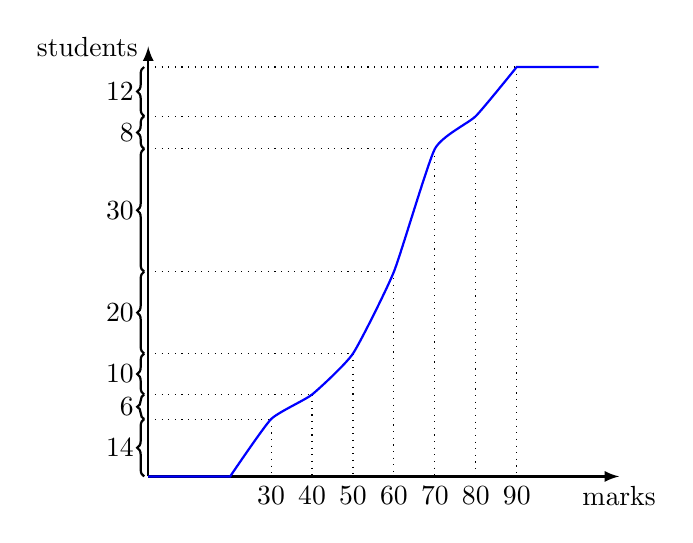
\begin{tikzpicture}[scale=0.052]
\draw[thick,-latex] (0,0) -- (115,0) node[below] {marks};
\draw[thick,-latex] (0,0) -- (0,105) node[left] {students};
\xdef\Lst{(20,0)}
\xdef\oldY{0}
\foreach \Y [count=\X] in {14,6,10,20,30,8,12}
{\pgfmathtruncatemacro{\newX}{10*(\X+2)}
\pgfmathsetmacro{\newY}{\oldY+\Y}
\draw[thick,decoration=brace,decorate] (-1,\oldY) -- (-1,\newY)
            node[midway,left]
            {\Y~};
\draw[dotted] (0,\newY) -- (\newX,\newY);
\draw[dotted] (\newX,\newY) -- (\newX,0) node[below]{\newX};
\xdef\oldY{\newY}
\xdef\Lst{\Lst (\newX,\newY)}
}
\xdef\Lst{\Lst}
\draw[blue,thick,smooth] (0,0) -- plot[smooth,tension=0.3] coordinates \Lst 
-- (110,100);
\end{tikzpicture}
\caption{Ogive}
\label{fig:ogive}
\end{figure}
\end{minipage}
\hspace{0.05\linewidth}
\begin{minipage}{0.45\linewidth}
\begin{figure}[H]
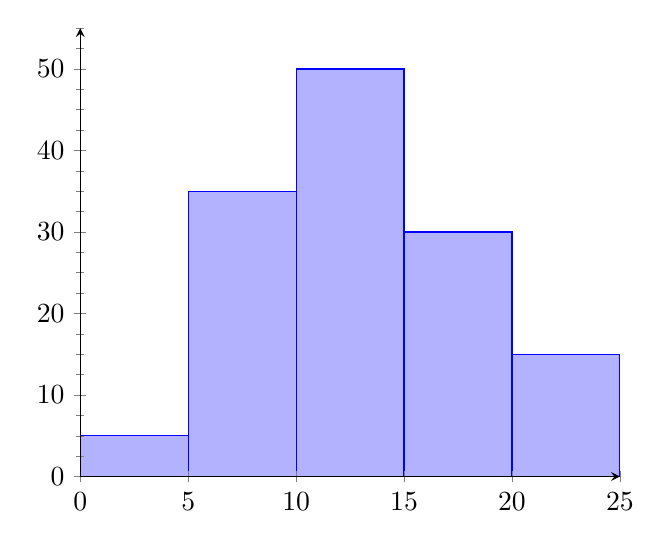
\begin{tikzpicture}
\begin{axis}[
    ymin=0, ymax=55,
    minor y tick num = 3,
    area style,
    axis lines=left,
    ]
\addplot+[ybar interval,mark=no] plot coordinates { (0, 5) (5, 35) (10, 50) (15, 30) (20, 15) (25, 0) };
\end{axis}
\end{tikzpicture}
\caption{Histogram}
\label{fig:hist}
\end{figure}
\end{minipage}
\end{minipage}

\vspace{1ex}

For data given to be:
57,94, 84, 63, 72, 51, 50, 48, 61, 71, 93, 82, 100, 89, 67, 78, 79, 78, 76, 85, 87, 73, 66, 99, 84, 72, 66

The stem-and-leaf diagram is:

\begin{table}[H]
\begin{center}
\begin{tabular}{|c|cccccccc|}
\hline
Stem &
  \multicolumn{8}{c|}{Leaf} \\ \hline
4 &
  \multicolumn{1}{c|}{8} &
  \multicolumn{1}{c|}{} &
  \multicolumn{1}{c|}{} &
  \multicolumn{1}{c|}{} &
  \multicolumn{1}{c|}{} &
  \multicolumn{1}{c|}{} &
  \multicolumn{1}{c|}{} &
   \\ \hline
5 &
  \multicolumn{1}{c|}{7} &
  \multicolumn{1}{c|}{1} &
  \multicolumn{1}{c|}{0} &
  \multicolumn{1}{c|}{} &
  \multicolumn{1}{c|}{} &
  \multicolumn{1}{c|}{} &
  \multicolumn{1}{c|}{} &
   \\ \hline
6 &
  \multicolumn{1}{c|}{3} &
  \multicolumn{1}{c|}{1} &
  \multicolumn{1}{c|}{7} &
  \multicolumn{1}{c|}{6} &
  \multicolumn{1}{c|}{6} &
  \multicolumn{1}{c|}{} &
  \multicolumn{1}{c|}{} &
   \\ \hline
7 &
  \multicolumn{1}{c|}{2} &
  \multicolumn{1}{c|}{1} &
  \multicolumn{1}{c|}{8} &
  \multicolumn{1}{c|}{9} &
  \multicolumn{1}{c|}{8} &
  \multicolumn{1}{c|}{6} &
  \multicolumn{1}{c|}{3} &
  2 \\ \hline
8 &
  \multicolumn{1}{c|}{4} &
  \multicolumn{1}{c|}{2} &
  \multicolumn{1}{c|}{9} &
  \multicolumn{1}{c|}{5} &
  \multicolumn{1}{c|}{7} &
  \multicolumn{1}{c|}{4} &
  \multicolumn{1}{c|}{} &
   \\ \hline
9 &
  \multicolumn{1}{c|}{4} &
  \multicolumn{1}{c|}{3} &
  \multicolumn{1}{c|}{9} &
  \multicolumn{1}{c|}{} &
  \multicolumn{1}{c|}{} &
  \multicolumn{1}{c|}{} &
  \multicolumn{1}{c|}{} &
   \\ \hline
10 &
  \multicolumn{1}{c|}{0} &
  \multicolumn{1}{c|}{} &
  \multicolumn{1}{c|}{} &
  \multicolumn{1}{c|}{} &
  \multicolumn{1}{c|}{} &
  \multicolumn{1}{c|}{} &
  \multicolumn{1}{c|}{} &
   \\ \hline
\end{tabular}
\end{center}
\caption{Stem-and-Leaf Diagram}
\label{fig:stemleaf}
\end{table}






\chapter*{Unit 2: Measures of Central Tendency}
\subsection*{What are they?}

\begin{itemize}
\item It is sometimes essential to condense
the data into a single value which can describe
the characteristics of the entire data
\item This single value is referred to as an average or central value or measure of central tendency
\item In practice, the word ‘average’ is used with different meanings
\item In some cases, we use term ‘average’ to denote a mediocre type e.g. average student, average film, average actor etc.
\item In some other cases, by ‘average’ we mean
‘typical’ or ‘usual’ e.g. average height of an
Indian, average income etc.
\item In statistics, ‘average’ refers to a value obtained by a specific process e.g. average height, average income etc.
\item In statistical terms, average is a value around which most of the observations in the data are clustered
\item It usually lies somewhere near the center of the group of observations and hence averages are termed as measures of central tendency
\item This single value depicts the main characteristics of the data
\item Large volumes of data cannot be easily understood or remembered
\item So, a single value summarizing prominent features of the data is needed
\item If two or more sets of data are to be compared, it is not possible to compare each and every item
\item So, we require a single value representing the entire data in condensed form
\item Thus, the objectives of a measure of central tendency or an average are:
\begin{itemize}
\item To obtain a single representative quantity for the entire data
\item To facilitate comparison
\end{itemize}
\item The most commonly used measures of central
tendency are:
\begin{enumerate}
\item Mean(s):
\begin{enumerate}[a.]
\item Arithmetic
\item Geometric
\item Harmonic
\end{enumerate}
\item Median
\item Mode
\end{enumerate}
\item The means are mathematical averages, while the median is a positional average
\end{itemize}

\subsection*{What makes a good average?}

\begin{itemize}
\item It should be simple to understand and easy to calculate
\item It should be rigidly defined
\item It should be based on all observations in the data and sensitive to changes
\item It should be capable of further mathematical treatment
\item It should be least affected by extreme observations or sampling fluctuations
\item It should be a true representative of the data
\end{itemize}

\subsubsection*{Properties, Merits and Demerits}
\begin{description}
\item[Arithmetic Mean]
\begin{description}
\item[]
\item[Properties]
\begin{itemize}
\item[]
\item If a constant is added or subtracted from each observations in the data, the A.M. of the data will be affected in the same way e.g. if each observation in the data is multiplied by 2, the A.M. of the new data will be two times the original A.M.
\end{itemize}
\item[Merits]
\begin{itemize}
\item[]
\item It is rigidly defined
\item It is easy to understand and easy to calculate
\item It is based on all the observations
\item It is capable of further algebraic treatment
\item Of all the averages A.M. is least affected by sampling fluctuations i.e., it is a stable average
\end{itemize}
\item[Demerits]
\begin{itemize}
\item[]
\item It cannot be obtained by mere inspection nor can it be located graphically
\item It cannot be obtained even if a single observation is missing
\item It is affected by extreme values
\item It cannot be calculated for frequency distribution having open end class intervals e.g. class-intervals like below 10, above 50, etc.
\item It may be a value which may not be present in the data
\item Sometimes, it gives absurd results e.g. average number of children per family is 1.28
\item It cannot be used for the study of qualitative data such as intelligence, honesty, beauty, etc.
\end{itemize}
\item Even though A.M. has various demerits, it is considered to be the best of all averages as it satisfies most of the requisites of a good average. It is called the \textbf{ideal average}.
\end{description}
\item[Median]
\begin{description}
\item[]
\item[Properties]
\begin{itemize}
\item[]
\item Median is the value of the central observation in the data when the observations are arranged in increasing (or decreasing) order of their magnitude.
\item It divides the data into two parts containing equal number of observations above and below it.
\end{itemize}
\item[Merits]
\begin{itemize}
\item[]
\item It is easy to understand and easy to calculate
\item It is quite rigidly defined
\item It can be computed for a distribution with open-end
classes.
\item In majority of the cases, it is one of the values in the data
\item It can be determined graphically
\item Since median is a positional average, it can be computed
even if the observations at the extremes are unknown
\item It is not highly affected by fluctuations in sampling
\item It can be calculated even for qualitative data.
\end{itemize}
\item[Demerits]
\begin{itemize}
\item[]
\item When the number of observations is large, the pre-requisite of arranging observations in ascending/descending order of magnitude is a difficult process.
\item It is not based on all observations and hence, may not be a proper representative.
\item It is not capable of further mathematical treatment.
\item Since it does not require information about all observations, it is insensitive to some changes.
\end{itemize}
\end{description}
\item[Mode]
\begin{description}
\item[]
\item[Properties]
\begin{itemize}
\item[]
\item Mode is defined as the value of the variable which occurs most frequently in the data
\item It is a value which is repeated maximum number of times or with high frequency
\item Thus, mode is considered as the most typical value of the data
\end{itemize}
\item[Merits]
\begin{itemize}
\item[]
\item It is easy to understand and simple to calculate.
\item It is not affected by extreme values or sampling fluctuations
\item It can be calculated for distribution with open-ended classes.
\item It can be determined graphically.
\item It is always present within the data and is most typical value of the given set of data
\item It is applicable to both qualitative and quantitative data
\end{itemize}
\item[Demerits]
\begin{itemize}
\item[]
\item It is not rigidly defined.
\item It is not based on all observations
\item It is not capable of further mathematical treatment
\item It is indeterminate if the modal class is at the extreme of the distribution
\item If the sample of data for which mode is obtained is small, then such mode has no significance.
\end{itemize}
\end{description}
\end{description}

\subsection*{Calculating these measures}

\subsubsection*{Arithmetic Mean}
\begin{description}
\item[Raw Data]
\[
\overline{x} = \frac{\text{Sum of Observations}}{\text{Number of Observations}} = \frac{x_1 + x_2 + \dots + x_n}{n} = \frac{\sum_{i=1}^n x_i}{n}
\]
\item[Ungrouped Frequency Distribution]
\[
\overline{x} = \frac{f_1 \cdot x_1 + f_2 \cdot x_2 + \dots + f_n \cdot x_n}{f_1 + f_2 + \cdot + f_n} = \frac{\sum_{i=1}^n f_i x_i}{\sum_{i=1}^n f_i}
\]
where \(f_i\)'s are the frequencies of each individual \(x_i\)'s.
\item[Grouped Frequency Distribution]
\[
\overline{x} = \frac{\sum_{i=1}^n f_i x_i}{\sum_{i=1}^n f_i}
\]
where \(x_i\)'s are the class marks of each individual class.
\item[Combined]
\[
\overline{x} = \frac{\sum_{i=1}^k n_i \overline{x_i}}{\sum_{i=1}^k n_i}
\]
where \(n_i\)'s are the population sizes of \(k\) populations, and \(\overline{x_i}\)'s are their respective population arithmetic means.
\item[Weighted]
\[
\overline{x} = \frac{\sum_{i=1}^n w_i x_i}{\sum_{i=1}^n w_i}
\]
where \(w_i\)'s are the weights of each individual \(x_i\)'s.
\end{description}

\subsubsection*{Geometric Mean}
\begin{description}
\item[Raw Data]
\[
G = \mathrm{antilog} \left[ \frac{\sum_{i=1}^n \log x_i}{n} \right]
\]
\item[Frequency Distribution]
\[
G = \mathrm{antilog} \left[ \frac{\sum_{i=1}^n f_i \log x_i}{n} \right]
\]
where \(f_i\)'s are the frequencies of each individual \(x_i\)'s, and \(x_i\)'s are the class marks of each individual class in case of grouped frequencies.
\end{description}

\subsubsection*{Harmonic Mean}
\begin{description}
\item[Raw Data]
\[
H = \dfrac{n}{\sum_{i=1}^n \left( \sfrac{1}{x_i} \right)}
\]
\item[Frequency Distribution]
\[
H = \dfrac{\ls{i}{n} f_i}{\ls{i}{n} \left( \sfrac{f_i}{x_i} \right)}
\]
where \(f_i\)'s are the frequencies of each individual \(x_i\)'s, and \(x_i\)'s are the class marks of each individual class in case of grouped frequencies.
\end{description}

\begin{align*}
\intertext{Let \(a\) and \(b\) be two positive numbers, and \(A\), \(G\), and \(H\) be their arithmetic, geometric, and harmonic means respectively.}
A &= \frac{a+b}{2} \\
G &= \sqrt{ab} \\
H &= \frac{2}{\sfrac{1}{a} + \sfrac{1}{b}} = \frac{2ab}{a+b} \\
A \cdot H &= \frac{a+b}{2} \cdot \frac{2ab}{a+b} \\
&= ab \\
&= G^2 \\
\implies G &= \sqrt{AH} \\
\intertext{Next,}
A - G &= \frac{a+b}{2} - \sqrt{ab} \\
&= \frac{1}{2} (a - 2\sqrt{ab} + b) \\
&= \frac{1}{2} (\sqrt{a} - \sqrt{b})^2 \\
&\ge 0 \\
\comment{i} \implies A &\ge G
\intertext{Also,}
G - H &= \sqrt{ab} - \frac{2ab}{a+b} \\
&= \frac{\sqrt{ab}}{a+b} (a - 2\sqrt{ab} + b) \\
&= \frac{\sqrt{ab}}{a+b} (\sqrt{a} - \sqrt{b})^2 \\
&\ge 0 \\
\comment{ii} \implies G &\ge H
\intertext{From (i), (ii),}
A \ge \ &G \ge H
\end{align*}

\subsubsection*{Median}
\begin{description}
\item[Raw Data]
\begin{itemize}
\item[]
\item[\(n\) \textbf{is odd}] The median is the \(\left( \frac{n+1}{2} \right)^\text{th}\) observation.

\item[\(n\) \textbf{is even}]  The median is the average of the \(\left( \frac{n}{2} \right)^\text{th}\) and \(\left( \frac{n}{2} + 1 \right)^\text{th}\) observation.
\end{itemize}


\item[Ungrouped Frequency Data]
\begin{enumerate}[Step 1.]
\item[]
\item Find less than type cumulative frequencies for the given ungrouped frequency distribution.
\item Find the total of the frequencies, say \(N = \sum f\).
\item If \(N\) is odd, find the value of the \(\left( \frac{n+1}{2} \right)^\text{th}\) observation. The median is that value of the variable at which the less than type cumulative frequency is equal to or exceeds \(\left( \frac{n+1}{2} \right)\) for the first time.
\item If \(N\) is even, find the value of the variable at which the less than type cumulative frequency is equal to or exceeds \(\left( \frac{n}{2} \right)\) and \(\left( \frac{n}{2} + 1 \right)\) for the first time. If these two values are same, this value is the median of the distribution. If the two values are different, the median is their arithmetic mean.
\end{enumerate}
\item[Grouped Frequency Data]
\begin{enumerate}[Step 1.]
\item[]
\item Find less than type cumulative frequencies.
\item Locate the median class (Median class is the class-interval in which the value of the median i.e. where the value of \(\frac{n}{2}^\text{th}\) observation falls). It is that class-interval where less than type cumulative frequency is equal to or
exceeds \(\frac{n}{2}\) for the first time.
\item The value of median (\(M\)) can then be calculated using the formula
\[
M = l_1 + \dfrac{(l_2 - l_1)(\sfrac{\mathrm{N}}{2} - \text{c.f.})}{\mathrm{f}}
\]
where,
\begin{description}
\item[\(l_1\)] lower class-boundary of the median class
\item[\(l_2\)] upper class-boundary of the median class
\item[\(\mathrm{c.f.}\)] less than type cumulative frequency of the pre-median class (i.e. the class interval just preceding to the median class)
\item[\(\mathrm{f}\)] frequency of the median class
\item[\(\mathrm{N}\)] total frequency
\end{description}
\end{enumerate}
\end{description}

\subsubsection*{Mode}
\begin{description}
\item[Raw Data and Ungrouped Frequency Distribution]
\begin{itemize}
\item[]
\item If the data is available in the form of individual observations, mode can be obtained by inspection or in case of large number of values after converting the data as an ungrouped frequency distribution.
\item For ungrouped frequency distribution, the mode can be determined merely by inspection as the value of the variable having the maximum frequency.
\end{itemize}
\item[Grouped Frequency Distribution]
\begin{enumerate}[Step 1.]
\item[]
\item Suppose the data is represented in the form of a continuous frequency distribution as class-intervals and corresponding frequencies. (If the given class-intervals are inclusive type, they must be converted to continuous or exclusive type before calculating the modal value.)
\item Then, locate the class-interval corresponding to the highest frequency. This class-interval is called as the modal class.
\item The mode can then be calculated by the following formula:
\[
M = l_1 + \frac{(l_2 - l_1)(f_1 - f_0)}{(f_1-f_0)+(f_2-f_1)}
\]
where,
\begin{description}
\item[\(l_1\)] lower class-boundary of the modal class
\item[\(l_2\)] upper class-boundary of the modal class
\item[\(f_1\)] frequency of the modal class
\item[\(f_0\)] frequency of the pre-modal class
\item[\(f_2\)] frequency of the post-modal class
\end{description}
\item The assumptions for this method are:
\begin{enumerate}[i.]
\item The frequency distribution must be continuous with exclusive type classes and having unique maximum frequency.
\item The width of all the class-intervals must be the same. In case of distribution with unequal class-intervals, they should be made equal under the assumption that frequencies are uniformly distributed over the classes.
\item Mode cannot be determined if the modal class is at the extreme i.e. the maximum frequency occurs at the beginning or at the end of the frequency distribution. To overcome this difficulty in computing mode, the empirical relationship Mean – Mode 3 (Mean – Median) can be used. The relationship holds for a moderately skewed unimodal
frequency distribution. This empirical relationship \textbf{cannot} be proved theoretically. Karl Pearson has stated it after observing it to be valid for a number of data sets by actual computations.
\end{enumerate}
\end{enumerate}
\end{description}

\subsection*{Quantiles}
The median of the data divides the series of observations/distributions into two parts containing equal observations. There are other values which also divide the series into a number of parts. These values are called as partition values or quantiles.
	
\begin{figure}[h!]
\centering
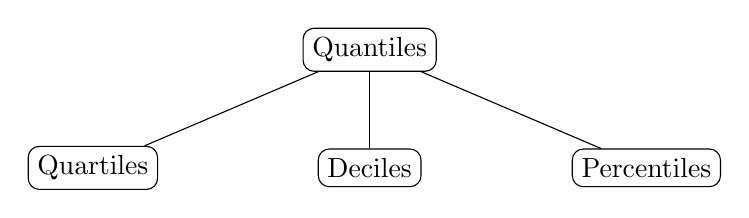
\begin{tikzpicture}
    [
      sibling distance=10em, 
      every node/.style = {shape=rectangle, rounded corners, draw, align=center, ->}
    ]

    \node{Quantiles}
      child {node{Quartiles}}
      child {node{Deciles}}
      child {node{Percentiles}
            };
\end{tikzpicture}
\caption{Basic Types of Quartiles}
\label{fig:quartiletypes}
\end{figure}

\begin{description}
\item[Quartiles]
\begin{itemize}
\item[]
\item The three values which divide the series into four parts, such that frequency of each part is 25\% of the total are called quartiles.
\item They are denoted by Q\(_i, i = 1, 2, 3\).
\item Similar to the median calculations, we simply replace \(\frac{N}{2}\) by \(\frac{iN}{4}\), where \(i = 1, 2, 3\) denote the quartile number. Its formula is also derived from the median formula where:
\[
\mathrm{Q}_i = l_1 + \dfrac{(l_2 - l_1)(\sfrac{\mathrm{iN}}{4} - \text{c.f.})}{\mathrm{f}}
\]
\end{itemize}
\item[Deciles and Percentiles]
\item The nine points which divide the series into 10 parts, such that frequency of each part is 10\% of the total, are called deciles.
\item Whereas, percentiles are ninety nine points which divide the series into 100 parts, where frequency of each part is 1\% of the total.
\item Thus, in particular, 6th decile will have 60\% observations below it and 40\% observations above it. 54th percentile will have 54\% observations below it and 46\% observations above it.
\item For raw data,
\(
\mathrm{D}_i = i\left(\frac{n+1}{10}\right)^\text{th}
\) observation,
\(
\mathrm{D}_i = i\left(\frac{n+1}{100}\right)^\text{th}
\) observation
\item The i\(^\text{th}\) decile and percentile formulae for grouped frequencies respectively now are:
\[
\mathrm{D}_i = l_1 + \dfrac{(l_2 - l_1)(\sfrac{\mathrm{iN}}{10} - \text{c.f.})}{\mathrm{f}}
\]
\[
\mathrm{P}_i = l_1 + \dfrac{(l_2 - l_1)(\sfrac{\mathrm{iN}}{100} - \text{c.f.})}{\mathrm{f}}
\]
\end{description}

\subsection*{Comparison of Different Central Measures of Tendency}
\begin{itemize}
\item We have studied five different measures of central tendency.
\item It is \textbf{obvious} that no single measure can be the best for all situations
\item The most commonly used measures are mean, median and mode.
\item It is not desirable to consider any one of them to be superior or interior in all situations.
\item The selection of appropriate measure of central tendency would largely depend upon the nature of the data; more specifically, on the scale of measurement for representing the data and purpose on hand.
\item The data obtained on nominal scale, we can count the number of cases in each category and obtain the frequencies
\item We may then be interested in knowing the class which is most typical value in the data.
\item In such cases mode can be used as the appropriate measure of
central tendency.
\item[\textbf{e.g.}] Suppose, in a genetical study, for a group of 50 family members, we want to know most common colour of eyes. Then we count the number of persons for each different colour of eye. Suppose 3 persons have light eyes, 6 persons have brown eyes, 12 with dark grey eyes and 29 persons are with black eyes. Then the more common colour of eyes (i.e. mode) for this group of people is ‘black’.
\item When the data is available on ordinal scale measurement i.e. the data is provided in rank order, use of median as a measure of central tendency is appropriate.
\item Suppose in a group of 75 students, 10 students have failed, 15 get pass class, 20 secure second class and 30 are in first class.
\item The average performance of students will be the performance of the middlemost student (arranged as per rank) i.e. the performance of 38\(^\text{th}\) student i.e. second class; which is the median of the data.
\item Median is only a point on the scale of measurement, below and above which lie exactly 50\% of the data.
\item Median can also be used (i) for truncated (incomplete) data, provided we know the total number of cases and their positions on the scale and (ii) when the distribution is markedly skewed
\item Arithmetic Mean is the most commonly used measure of central tendency.
\item It can be calculated when the data is complete and is represented on interval or ratio scale.
\item It represents the centre of gravity of the data i.e. the measurement in any sample are perfectly balanced about the mean.
\item In computation of simple A. M. equal importance is given to all observations in the data.
\item It is preferred because of the its high reliability and its applicability to inferential statistics.
\item Thus, A. M. is the more precise, reliable and stable measure of central tendency.
\item Geometric mean is appropriate measure of central tendency when data is related to ratios, rates and percentages.
\item It is usually used to obtain average percentage change in any characteristics.
\item Geometric mean is best to be used when one wants to give more weights to small values than large values in the series
\item Harmonic mean, like geometric mean, is also a measure of central tendency used in solving special types of problems.
\item It is generally used for averaging speed, prices. etc.
\item We have seen that each measure of central tendency has situations for its best use and also has its own limitations.
\item So one has to take conscious decision about its applicability.
\item Selection of appropriate measure of central tendency requires experience and insight to examine the nature of data and purpose in hand.
\end{itemize}

\chapter*{Unit 3: Measures of Dispersion, Skewness and Kurtosis}

\subsection*{What makes a good measure of dispersion?}

\begin{itemize}
\item It should be easy to calculate and simple to understand
\item It should be rigidly defined
\item It should be based on all observations
\item It should be capable of further algebraic treatment
\item It should have sampling stability
\item It should not be unduly affected by extreme values
\item We shall now study the various absolute and relative measures of dispersion.
\end{itemize}

There are two types of measures to look at.
\begin{description}
\item[Absolute Measures] Range, Quartile Deviation or Semi-inter Quartile Range, Mean Deviation and Standard Deviation.
\item[Relative Measures] Coefficient of Range, Coefficient of Quartile Deviation, Coefficient of Mean Deviation and Coefficient of Variation.
\end{description}

\begin{description}
\item[Range]
\begin{itemize}
\item[]
\item If L is the largest observation in the data and S is the smallest observation, then
\[\text{Range} = L - S\]
\item For a frequency distribution, range may be considered as the difference between the largest and the smallest class boundaries \item Range is crude, and the simplest measure of dispersion. It measures the scatter of observations among themselves and not about any average.
\item The corresponding relative measure is \
\[\text{Coefficient of Range} = \frac{L-S}{L+S}\]
\item Range is a suitable measure of dispersion in case of small groups.
\item In the branch of statistics known as Statistical Quality Control, range is widely used.
\item It is also used to measure the changes in the prices of shares.
\item Variation in daily temperatures at a certain place are measured by recording maximum temperature and minimum temperature.
\item Range is also used in medical sciences to check whether blood pressure, haemoglobin count, etc. are normal.
\item The main drawback of this measure is that it is based on only two extreme values, the maximum and the minimum and completely ignores all the remaining observations.x
\end{itemize}
\item[Quartile Deviation]
\begin{itemize}
\item[]
\item We have seen earlier that range, as a measure of dispersion, is based only on two extreme values and fails to take into account the scatter of the remaining observations within the range.
\item To overcome this drawback to an extent, we use another measure of dispersion called Inter- Quartile Range. It represents the range which includes the middle 50\% of the distribution. Hence,
\[\text{Inter-Quartile Range} = \mathrm{Q}_3 - \mathrm{Q}_1\]
where Q\(_3\) and Q\(_1\) represent the upper and lower quartiles respectively.
\[
\text{Semi-Inter-Quartile Range} = \text{Quartile Deviation} = \frac{\mathrm{Q}_3 - \mathrm{Q}_1}{2}
\]
The SIQR or Quartile Deviation is often used.
\item The corresponding relative measure is
\[ \text{Coefficient of Quartile Deviation} = \frac{\mathrm{Q}_3 - \mathrm{Q}_1}{\mathrm{Q}_3 + \mathrm{Q}_1} \]
\item Q.D. is independent of extreme values. It is better representative and more reliable than range.
\item Q.D. gives an idea about the distribution of middle half of the observations around the median.
\item Whenever median is preferred as s measure of central tendency, quartile deviation is preferred as a measure of dispersion. However, like median, quartile deviation is also not capable of further algebraic treatment, as it does not take into consideration all the values of the distribution.
\item For a symmetric distribution,
\begin{align*}
\mathrm{Q}_1 &= \text{Median} - \text{Q.D.} \\
\mathrm{Q}_3 &= \text{Median} + \text{Q.D.}
\end{align*}
\end{itemize}
\item[Mean Deviation]
\begin{itemize}
\item[]
\item Mean Deviation is defined as the arithmetic mean of the absolute deviations of the observations from any suitable constant, say \(A\).
\item Thus, if a variable \(X\) can assume values \(X_1, X_2,\dots, X_n\) and \(A\) is any arbitrary constant, then mean absolute deviation or mean deviation from \(A\) is defined as
\[\frac{\sum_{i=1}^n | X_i - A |}{n}\]
\item For a frequency distribution,
\[\frac{\sum_{i=1}^n f_i \cdot | X_i - A |}{n}\]
\item Though \(A\) is an arbitrarily selected constant, generally for statistical analysis it is taken as one of the measures of central tendency such as mean, median or mode. It is observed that M.D. from \(A\) is minimum when \(A\) is the median.
\item M. D. is the simplest measure of dispersion that takes into account all the values in a given distribution. However, it has some limitations as well. First, as it takes into account the absolute deviations (i.e. does not consider signs of the deviations),  it is unwieldy in mathematical operations. Secondly, it is influenced by extreme values.
\item The M. D. is useful in statistical analysis of economic and social phenomena, using small samples.
\end{itemize}
\item[Standard Deviation]
\begin{itemize}
\item[]
\item Standard Deviation (\(\sigma\)) is defined as the positive square root of the arithmetic mean of the square of the deviations of the observations from their arithmetic mean.
\item The arithmetic mean of the squares of the deviations of the observations from their A. M. is called the variance.
\[\sigma = \sqrt{\text{Variance}}\]
\begin{align*}
\intertext{For raw data,}
\sigma &= \sqrt{\dfrac{\ls{i}{n} (x_i - \overline x)^2}{n}}
\intertext{For ungrouped frequency distributions,}
\sigma &= \sqrt{\dfrac{\ls{i}{k} f_i \cdot (x_i - \overline x)^2}{\ls{i}{k} f_i}},\\ &{\overline{x} = \frac{\ls{i}{k} f_i \cdot x_i}{\ls{i}{k} f_i}}
\intertext{For grouped frequency distributions,}
\sigma &= \sqrt{\dfrac{\ls{i}{k} f_i \cdot (x_i - \overline x)^2}{\ls{i}{k} f_i}},\\ &{\overline{x} = \frac{\ls{i}{k} f_i \cdot x_i}{\ls{i}{k} f_i}, \ x_i\text{'s are the class marks.}}
\end{align*}
\item The corresponding relative measure is
\[\text{Coefficient of Variance} = \frac{\sigma}{\overline{x}}\]
\end{itemize}
\end{description}

\paragraph*{Properties of Standard Deviation}
\begin{description}
\item[Effect of change of origin and scale]
\[\text{If } u = \frac{x - a}{c}, \ \sigma_u = \frac{\sigma_x}{c}\]

\item[Standard Deviation for Combined Group]
For two populations with sizes \(n_1, n_2\), arithmetic means \(\overline{x_1}, \overline{x_2}\), and standard deviations \(\sigma_1, \sigma_2\),
\[ \overline{x} = \frac{n_1 \overline{x_1} + n_2 \overline{x_2}}{n_1 + n_2} \]
let \(d_1 = \overline{x_1} - \overline{x}\), \(d_2 = \overline{x_2} - \overline{x}\)
then,
\[\sigma = \sqrt{\frac{n_1(\sigma_1^2+d_1^2)+n_2(\sigma_2^2+d_2^2)}{n_1+n_2}}\]

\item[Zero Variance] If all observations in a series are equal or if the data contains only one observation, i.e. there is no variation in data, \(\sigma=0\).

\item[Spread] The spread of variable is approximately taken as (\(\overline{x} \pm 3 \sigma\)).

\item[Merits]
\begin{itemize}
\item[]
\item It is rigidly defined
\item It is based on all observations
\item It is capable of further algebraic treatment
\item It is least affected by sampling fluctuations
\end{itemize}

\item[Demerits]
\begin{itemize}
\item[]
\item As compared to other measures, it is difficult to calculate
\item It cannot be calculated for distribution with open end class-intervals
\item It gives more importance (weightage) to extreme values and less importance to the values close to A. M. i.e. it is affected due to extreme observations.
\item It cannot be calculated for qualitative data
\end{itemize}
\end{description}

\subsection*{Moments}
There are two types of moments,
\begin{description}
\item[Raw Moments] the deviations are taken from some constant
\item[Central Moments] the deviations are taken from A. M. of the distribution
\end{description}
In general, if a variable \(X\) takes values \(X_1, X_2, \dots X_n\),
then the \(r^\text{th}\) raw moment (\(\mu'_r\)) about the arbitrary origin \(a\) is calculated as
\[\mu'_r = \frac{\ls{i}{n} (x_i-a)^r}{n} \equiv \overbrace{\frac{\ls{i}{n} f_i  (x_i-a)^r}{\ls{i}{n} f_i}}^{\text{For frequency distributions}}\]

Raw moments with \(a=0\) are:
\[\mu'_r = \frac{\ls{i}{n} x_i^r}{n} \equiv \overbrace{\frac{\ls{i}{n} f_i  x_i^r}{\ls{i}{n} f_i}}^{\text{For frequency distributions}}\]

And the \(r^\text{th}\) central moment (\(\mu_r\)) is
\[\mu'_r = \frac{\ls{i}{n} (x_i-\overline{x})^r}{n} \equiv \overbrace{\frac{\ls{i}{n} f_i  (x_i-\overline{x})^r}{\ls{i}{n} f_i}}^{\text{For frequency distributions}}\]

Special Cases:
\begin{itemize}
\item \(\mu'_1 = \overline{x}\)
\item \(\mu_1 = 0\)
\item \(\mu_2 = \sigma^2 = \mu'_2 - {\mu'_1}^2\)

\subsection*{Skewness}

The property of any deviation of frequency distribution from symmetry is known as skewness. A distribution which is not symmetrical is called a skewed distribution. The distributions representing number of accidents per day, age of individuals, number of misprints per page etc. are generally non symmetric. In case of a skewed distribution; the observations are not symmetrical placed about the average, but there are more observations on one side of the average than on the other side. Also, the mean, median and mode of the distribution do not coincide, and the quartiles are not equi-spaced.

A frequency distribution is symmetric about some point \(x=a\), if the spread of frequencies on both sides of \(a\) is the same. This means that if a frequency curve of such a distribution is folded on the ordinate \(x = a\), the two halves of the curve will coincide with each other.

Types of Skewness:
\begin{description}
\item[Symmetric]
\begin{itemize}
\item[]
\item For a symmetric distribution, the values of mean, median and mode coincide, and also the lower and upper quartiles are equi-spaced from the median.
\item A symmetric distribution has zero skewness.
\end{itemize}
\item[Positive]
\begin{itemize}
\item If the density of observations is more for the lower values of the variable than for higher values of the variables, then the frequency curve increases rapidly to reach the maximum and further decreases slowly.
\item The tail of the frequency curve is elongated towards the right hand side.
\item Mean > Median > Mode, Q\(_3\) - Q\(_2\) > Q\(_2\) - Q\(_1\),
\item \(\mu_3 > 0\)
\item The distribution of income of individuals, house-rent, profits of companies etc. are usually positively skewed.
\end{itemize}
\item[Negative]
\begin{itemize}
\item[]
\item If the density of observations is more for higher values of the variable than for lower values of the variable
\item The tail of the frequency curve is elongated towards the left side.
\item Mean < Median < Mode, Q\(_3\) - Q\(_2\) < Q\(_2\) - Q\(_1\),
\item \(\mu_3 < 0\)
\item The distribution of supply with respect to price, numbers of depositors with respect to savings in the bank are usually negatively skewed.
\end{itemize}
\end{description}
\end{itemize}

\paragraph*{Absolute Measures of Skewness}
\begin{description}
\item[Pearson's Measure]
\[ = \text{Mean} - \text{Mode} \]
\item[Bowley's Measure]
\[ = (\mathrm{Q}_3 - \mathrm{Q}_2) - (\mathrm{Q}_2 - \mathrm{Q}_1)) \]
\end{description}

\paragraph*{Relative Measures of Skewness}
\begin{description}
\item[Pearson's Coefficient]
\[\text{SK}_\text{p} = \frac{\text{Mean} - \text{Mode}}{\sigma} \]
If \(\text{SK}_\text{p}\) is positive, the data is positively skewed, and vice versa.
\item[Bowley's Coefficient]
\[\text{SK}_\text{B} = \frac{\mathrm{Q}_3+\mathrm{Q}_1 - 2\mathrm{Q}_2}{\mathrm{Q}_3 - \mathrm{Q}_1} \]
If \(\text{SK}_\text{B}\) is positive, the data is positively skewed, and vice versa. Also, \(|\text{SK}_\text{B}|<1\).
\item[Relative Measure based on Moments]
\[\beta_1 = \dfrac{\mu_3^2}{\mu_2^3}, \gamma_1 = \sqrt{\beta_1} \]
If \(\gamma_1 = 0\), the distribution is symmetric. \\
If \(\gamma_1 > 0\), the distribution is positively skewed.\\
If \(\gamma_1 < 0\), the distribution is negatively skewed.\\
\end{description}

\subsection*{Kurtosis}

Kurtosis is the other important aspect of a curve which refers to its degree of flatness or peakedness. The frequency curves of different distributions have different degree of flatness or peakedness about the mode. If the spread of the observations in a distribution is less, then there is more concentration of observations around mode and the frequency curve of such a distribution will have a taller peak as compared to the frequency curve of a distribution having more spread. In short, frequency curves can be broadly categorized as of three different types with regard to the convexity, the property which is referred to as \textbf{Kurtosis}.

The kurtosis of a bell shaped curve (of normal distribution) is taken as standard. Such as curve is neither peaked nor flat-topped and is called a 'mesokurtic' curve. A curve which is more flat-topped than normal curve is called 'platykurtic' and a curve which is more peaked than the normal curve is called as 'leptokurtic'.

\paragraph*{Measures of Kurtosis}
\textbf{Relative Measure Based on Moments}
\[\beta_2 = \frac{\mu_4}{\mu_2^2}, \gamma_2 = \beta_2 - 3\]
If \(\gamma_2 = 0, \beta_2 = 3\), the distribution is mesokurtic. \\
If \(\gamma_1 > 0, \beta_2 > 3\), the distribution is leptokurtic.\\
If \(\gamma_1 < 0, \beta_2 < 3\), the distribution is platykurtic.\\

\paragraph*{Box-and-Whisker Plot}


A box and whisker display (a.k.a. boxplot) is another graphic technique used in Exploratory Data Analysis. It shows the five number summary for a univariate data set, giving a quick impression of the distribution. The five number summary is defined as a set of five landmark points of a data viz. smallest data value, lower quartile, median, upper quartile and the largest data value.

\begin{enumerate}[Step 1.]
\item To construct a horizontal box and whisker diagram, draw a horizontal axis that is scaled to the data. Above the axis, draw a rectangle box of convenient height with the left side (or left hinge) and right side (or right hinge) at Q\(_1\) and Q\(_3\) respectively. 
\item Draw a vertical line segment at Q\(_2\). The length of this box is then equal to Q\(_3\) - Q\(_1\) i.e. the interquartile range (IQR).
\item Then, two sets of limits viz. inner fence and outer fence are calculated as (Q\(_1 - 1.5 \times\) IQR), (Q\(_3 + 1.5 \times\) IQR) and (Q\(_1 - 3 \times\) IQR), (Q\(_3 + 3 \times\) IQR) respectively. 
\item Two lines are drawn outside the box parallel to horizontal axis, one from the midpoint of the left side of the box to the smallest value inside lower limit of inner fence and the other from the midpoint of the right side of the box to the largest value inside upper limit of the inner fence.
\item These two lines are termed as the left whisker and right whisker respectively.
\end{enumerate}

Sometimes, the given data is such that few observations are much larger or much smaller than most of the observations. Such observations are called outliers are usually indicated by special symbols such as * on the box plot. Such observations, if they lie between inner and outer fence, are called suspected outliers. The observations beyond the outer fence are called outliers.

The box and whisker display can show, at a glance, whether the given data set is reasonably symmetrical or skewed. A median line that is approximately in the centre of the box indicates that the data is reasonably symmetric. But a median line towards the right side of the box indicated negative skewness, while a median line towards the left of the box suggests positive skewness. Also, skewness is indicated if one whisker line is appreciably longer than the other Box-plots are useful for comparing several groups of numbers.

%----------------------------------------------------------------------------------------

\end{document}
